%----------------------------------------------------------------
%
%  File    :  survey-intro.tex
%
%  Author  :  Keith Andrews, IICM, TU Graz, Austria
% 
%  Created :  27 May 1993
% 
%  Changed :  16 Nov 2010
% 
%----------------------------------------------------------------


\chapter{Introduction}

\label{chap:Intro}

Going back, at the starting point of web development, its creators
and designers have not had the need to think about the look and design
of the page, because back then, their users and clients would mostly access
the site via the same device, that being a personal desktop computer which would
mostly share the same resolution and display size. That means that they mostly
needed to design and work around the same concept. Also, they didn’t need to think
about things like what if an user entered the site with this device or this, so
they could basically use static and fixed positioning of elements.

However, todays' technologies, be it the mobile industry or technical industry
in general, the devices have come a long way, and are being worked on really
fast. What does that mean is that the programmers and designers need 
to consider that people will have different ways of using and browsing their 
pages, which require different approaches to design their web pages.
Nowadays, the clients and users have a broad list of devices, which they can use
to access a web page, be it a tablet, mobile phone, laptop and even TVs[1][2].    

Basically, the most important thing is to make the web pages' user interface 
as friendly as possible, so that the user does not lose much time navigating around.
And with that being said, web programmers need to automatically think about
making the web pages in that way, while they are being accessed from those different
devices mentioned[2].

Responsive Web Design is an approach, or more rather a technique, which is used
to construct a self-adapting web page, meaning that it adapts, resizes, shrink
and changes its' form in any way needed to perfectly fit the web-accessing device
used to visit it[3].   





\section{How to achieve Responsive Web Design}

If a programmer wants his web site to be responsive, he has to use 
following techniques:

$\bullet$ Media queries 

$\bullet$ Flexible images and media

$\bullet$ Fluid grid layouts



\section{Media queries}

Media queries are very important because with them it is possible to specify 
with what device the web page is being accessed. The query usually is made of
a media type, and some conditions which can check if the media type has some special
property.
\\
\\
\begin{lstlisting}[%
    language = CSS, 
    float=tp,
    xleftmargin=0cm,              % no extra margins for floats
    xrightmargin=0cm,             % no extra margins for floats
    language=biblatex,
    basicstyle=\footnotesize\ttfamily,
    frame=shadowbox,
    numbers=left,
    label=list:BibACMIEEE,
    ,
]
    % An example of a media query, where one can say that for a screen of size 850px or less, the background is black:

    @media screen and (max-width: 600px) {
    body   {
          background-color: olive;
        }
    }
\end{lstlisting}
Basically it allows defining specific CSS rules, depending on the device used.

From this example above, with the help of the parameter \emph{screen}
the media type was specified and using \emph{max-width} the condition was determined which
affects the device of the user. Now, there are many different conditions which
can be used, and they are really helpful, because with them it is possible to adjust 
display settings for every device there is. 

For example, if the user is entering the website with his phone, it can be automatically said that an image should have a lower resolution,
thus adjusting it better for his screen and saving some bandwith.

Another example would be using \emph{display:none} with which some content can completely be hidden that should not be 
displayed.

\begin{lstlisting}[%
    language = HTML, 
    xleftmargin=0cm,              % no extra margins for floats
    xrightmargin=0cm,             % no extra margins for floats
    language=biblatex,
    basicstyle=\footnotesize\ttfamily,
    frame=shadowbox,
    numbers=left,
    label=list:BibACMIEEE,
     stringstyle=\color{blue}
    ,
]
    % An example of using display: none:

    <!DOCTYPE html>
    <html>
    <head>
    <style>
    h1.none {
      display: none;
    }
    </style>
    </head>
    <body>

    <h1 class="none">This will not be displayed</h1>

    </body>
    </html>

\end{lstlisting}




%
If this was ran in the browser, header would not be seen, because
it was decided to not be shown. If \emph{display:none} was changed to \emph{display:block}
our header would be visible.

Include a list of \emph{all} the relevant papers and resources you
have found and mark those you have chosen to focus on. Make sure
\emph{all} the papers and resources you found or were given appear in
the bibliography.




\section{Fluid Grid Layouts}

Normally, websites are constructed in a layout which is grid-built, because they are
easier to handle in different kind of devices. Also what is specific
for that kind of layout is that it is built using divs, HTML tables and so on. Now, on top of that
responsive web design comes in play[5]. With it, it is possible to use percentage-based element sizing which is easier than using pixels. 

According by (Abdulrehman,2015) a flexible grid-layout is one of the foundations of responsive
design. Using the term "grid" does not mean necessarily that a grid framework needs to be used.
What it means is that specific CSS tricks are used for positioning. Also, he suggest that 
using pixels for the measurement unit should be stopped, because pixels can vary. 

For example, on one device they can be one point or dot, on another device it can be a few more, and therefore
unreliable. So, what needs to be done is that, if pixels are used, they should be converted using
a formula stated by (Marcotte, 2010) in  Dan Cederholm's book named "Handcrafted CSS":

\begin{ceqn}
\begin{align}
    Target \div Context = Result
\end{align}
\end{ceqn}

It is asserted by (Pettit, 2012) that, to use this formula, the context of the element
needs to be divided by the target element.
%TODO -> Example and how to achieve/use Fluid Grid Mirza



\section{Flexible images and media}

With this approach, any type of media,images depending on the screen resolution
will resize,collapse,crop and adjust accordingly to it, and to achieve this
it is possible to use the same thing mentioned in the previous section, relative units,
if the screen becomes too small then hide the image completely or by cropping some parts
of the image, again in the case if the screen becomes too small[6].

\subsection{Relative measurements} 

Instead of using pixels,relative dimensions can be used, percentage based. So instead of
specifying the view and dimensions in pixels, one can specify for example 60\%, which would result
in resizing or reshrinking of the image based on the resolution of the device accordingly to fill
60\% of the page. 

%\begin{figure}[h!]
  %  \centering
  %  \includegraphics[keepaspectratio,width=\linewidth,height=\halfh]
  %  {relative.png}
    
  %  \caption[Relative Image]{
  %  The web site of the TeX Users Group \parencite{TUG}.
    
   % \label{fig:TUG}
    %\end{figure}
    \begin{figure}[h!]
        \centering
        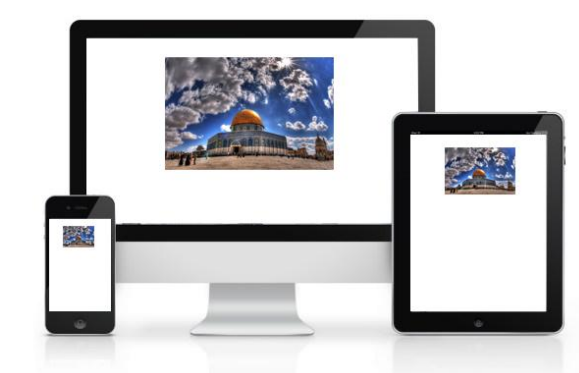
\includegraphics[keepaspectratio,width=\linewidth,height=\halfh]
        {relative.png}
        
        \caption[Relative Image Dimensions]{
            Relative Image Dimensions.
        \imgcredit{Taken from research paper.}
        }
        \label{fig:TUG}
        \end{figure}
%TODO SPECIFY LINK AL NE RADI MAMU MU
\newpage
\subsection{Cropping} 

Another option is cropping, which crops the picture to a certain width
with the help of CSS. 

\begin{figure}[h!]
    \centering
    \subfloat[%  the % chars remove implicit spacing
    Picture with original size
    ]
    {%
    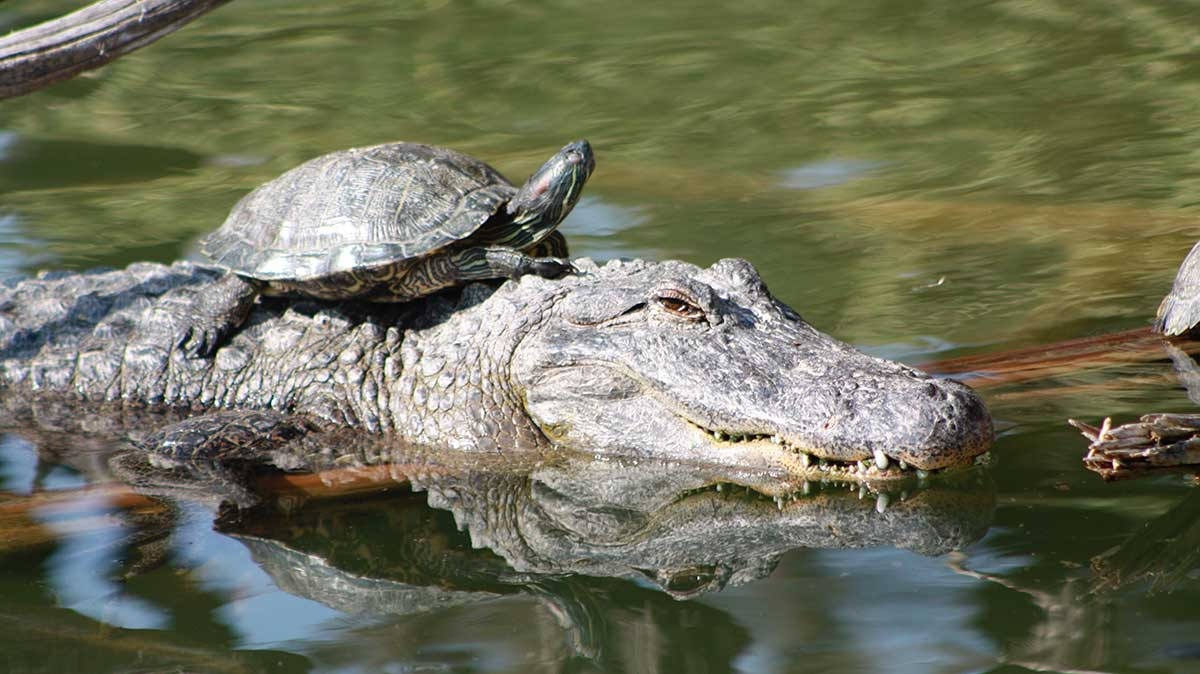
\includegraphics[width=\linewidth]
    {alig1.jpg}%
    \label{alig1}%
    }
    \hfill
    \subfloat[%
    Picture when cropped 
    ]
    {%
    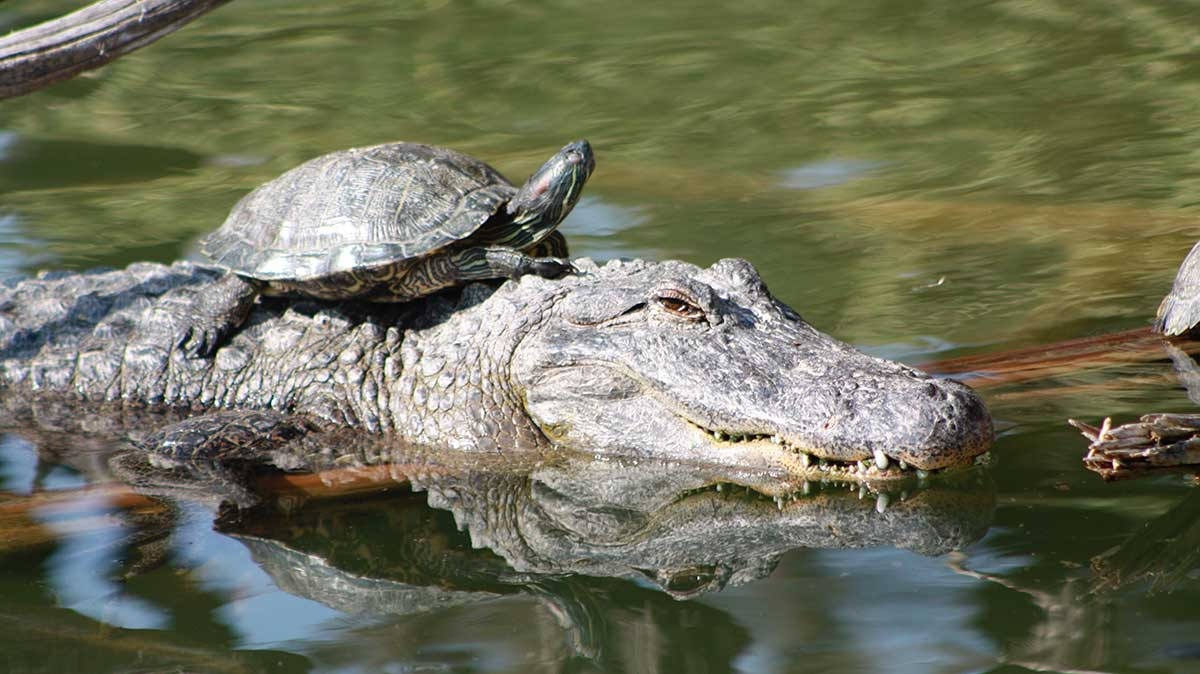
\includegraphics[width=0.45\linewidth]
    {alig2.jpg}%
    \label{alig2}%
    }
    
    \caption[Abstract Clock Towers]
    {
      Image cropping.
    \imgcredit{https://alligator.io/css/cropping-images-object-fit/.}
    }
    \label{figWhol}
\end{figure}

In this Figure above, it can be obviously seen that the result of tweaking the image a bit.
With just a few CSS commands, it is possible to crop the picture and if someone is browsing the
web site with a smaller device, the image does not have to be hidden, just its' size is changed.

\begin{lstlisting}[%
    language = HTML, 
    xleftmargin=0cm,              % no extra margins for floats
    xrightmargin=0cm,             % no extra margins for floats
    language=biblatex,
    basicstyle=\footnotesize\ttfamily,
    frame=shadowbox,
    numbers=left,
    label=list:BibACMIEEE,
     stringstyle=\color{blue}
    ,
]
    % An example of a media query, where one can say that for a screen of size 850px or less, the background is black:

    figure{
     width:300px; /*container-width*/
     overflow:hidden; /*hide bounds of image */
     margin:0;   /*reset margin of figure tag*/
   }
   figure img{
     display:block; /*remove inline-block spaces*/
     width:100%; /*make image streatch*/
}
\end{lstlisting}
Taken from
\imgcredit{https://medium.com/@elad/how-to-crop-images-with-css-b8471d402b16.}   